\chapter{Introduction to Programming in Opus for Modelers}
\label{app:python-overview}

This chapter provides a gentle introduction to programming in Opus.  It
is intended not for software developers but for model users, who need
to understand enough about the underlying software to be able to use
all of the capabilities of the system, and to extend these
capabilities.  

\section{Python}
\label{sec:python}

Python is a programming language developed initially by Guido van Rossum, and has become a very popular programming language with a large user and developer base.  It has been adopted, for example, by ESRI as the main scripting language for ArcGIS. It is Open Source software, and is available from www.python.org.  Python is an interpreted language, as compared to a compiled language.  This means that when you start Python, you are launching the Python interpreter, which then interacts with commands typed in interactively, or with programs (scripts) loaded from disk. 

Python can be launched in several ways:

\squishlist
\item from the command shell by typing \verb#python#, or from the start menu in Windows
\item from IDLE, a light-weight Python Editor and Shell that comes with Python, which can be launched from the start menu
\item using Scite, an editor that can also run Python programs
\item using a sophisticated Integrated Development Environment (IDE) sush as Eclipse, Wing, or Eric
\squishend

To get started, launch IDLE from the Windows \verb#Start# menu.  It will launch a window as shown in Figure \ref{fig:python-idle}.  If you are not on a Windows computer, just start a command shell and type \verb#python# to start an interactive Python session.

\begin{figure}[htp]
\begin{center}
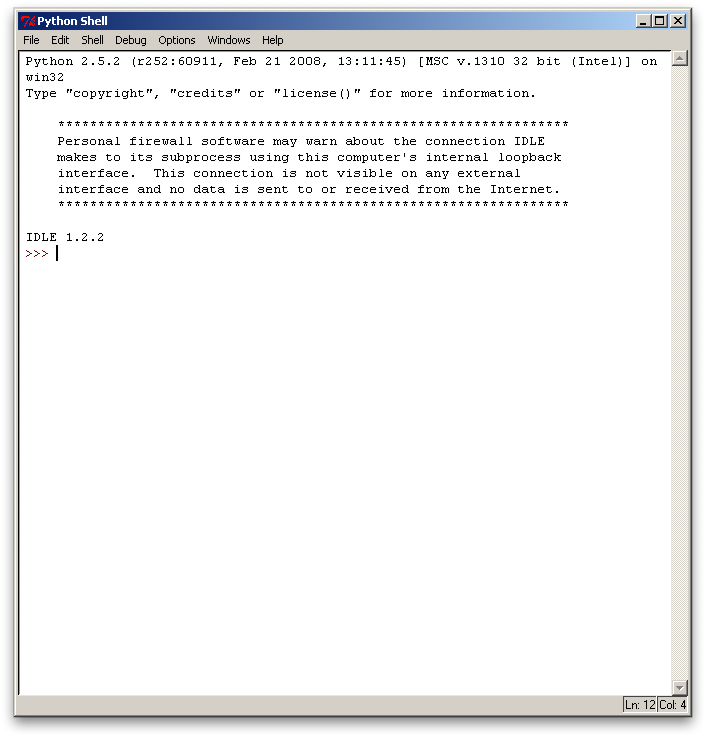
\includegraphics[scale=0.4]{graphics/python-idle.png}
\end{center}
\caption{The IDLE Python Shell}
\label{fig:python-idle}
\end{figure}

\subsection{Expressions and Data Types}

Python has several data types that are useful to understand as you begin to explore the language.  These data types are:

\squishlist
\item integers
\item floats
\item booleans
\item strings
\item tuples
\item lists
\item dictionaries
\squishend

Begin with the basics.  Python can do simple (or complex) calculations interactively, just as you might do with a calculator.  How might you compute the sum of two numbers?  Just type in a mathematical expression, and hit return.  Try 2+2, and 3/2.  Notice that the second answer is probably not what you want: the result is an integer, rather than a floating point, so it truncates.  To get a floating point result, use a decimal place on at least one of the inputs.\\

\begin{lstlisting}
>>> 2+2
4
>>> 3/2
1
>>> 3/2.0
1.5
\end{lstlisting}

The results of expressions are easily assigned to a variable name, and used in further calculations.  Notice that when you type an assignment of an expression to a variable, it does not print the value, but does assign it.  You can print or use the value at this point.  \\

\begin{lstlisting}
>>> a = 2+2
>>> a
4
>>> b = 3/2.0
>>> a+b
5.5
>>> (a+b)/2
2.75
\end{lstlisting}

Now examine what happens if we use operators that \verb#assert# a statement that can be evaluated as \verb#True# or \verb#False#.  This generates a \verb#Boolean# data type.

\begin{lstlisting}
>>> a = 2
>>> b = 4/2
>>> a == b    #This asserts that a is equal to b, by using == instead of =
True
>>> a < b      #This asserts that a is less than b
False
\end{lstlisting}

We have seen so far three of Python's data types: integers, floats, and booleans.  Text is also managed in Python, using its string datatype.  Strings can be assigned to variables, and used, for example to concatenate two strings, or to extract a portion of a string using the index.  Note that Python uses index values starting from 0.  If a single index value is used, then it identifies a single value in the string at the index position.  If two values are used, the second identifies the ending index value.  One behavior that is not intuitive is that the returned values are up to, but do not include the second index value.\\

\begin{lstlisting}
>>> a = 'Conca'
>>> b = 'tenate'
>>> c = a+b
>>> c
'Concatenate'
>>> c[0]
'C'
>>> c[0:2]
'Co'
>>> c[2:]
'ncatenate'
\end{lstlisting}

There are three other data types in Python that are closely related: tuples, lists and dictionaries.  Tuples contain a set of items that are indexed (like strings, above), but cannot be changed once defined.  An example would be the days of the week, or the months of the year:

\begin{lstlisting}
>>> days = ('Monday', 'Tuesday', 'Wednesday', 'Thursday', 'Friday', 'Saturday', 'Sunday')
>>> days[3]
'Thursday'
\end{lstlisting}

Lists are almost the same as tuples, but they can easily be modified, and items can be added or removed. A To Do list would be an example:

\begin{lstlisting}
>>> todo = ['get groceries', 'do homework', 'paint wall', 'watch movie']
>>> todo[1]
'do homework'
>>> todo.append('read book')
>>> todo
['get groceries', 'do homework', 'paint wall', 'watch movie', 'read book']
>>> del todo[1]
>>>todo
['get groceries', 'paint wall', 'watch movie', 'read book']
\end{lstlisting}

Dictionaries are flexible data structures that store key:value pairs, like a standard dictionary stores words and their associated definitions.  Entries can be looked up by their key.  A phonebook provides a simple example.  Note the syntax to add an entry.  Also, pay attention to the use of different kinds of brackets for these different data types.  They do matter, and will generate an error if the wrong one is used.

\begin{lstlisting}
>>> myPhoneBook = {'Mark':2439503, 'Julie':4309302, \
... 'Jeff':3540693}
>>> myPhoneBook['Jeff']
3540693
>>> myPhoneBook['Mary'] = 3339999
>>> myPhoneBook
{'Julie': 4309302, 'Jeff': 3540934, 'Mary': 3339999, 'Mark': 2439503}
\end{lstlisting}

\subsection{Python Modules, Packages, and Methods}

Python commands can be used interactively, as we have just seen,  but they can also be stored in a file, called a Python Module, provided that it ends with an extension of \verb#.py#, and follows some basic formatting requirements, like the use of indentation to identify what statements belong in a block.  More on this later.

Any Python statements you can execute interactively can be put into a Python module and then executed at the command line or loaded into IDLE or another program that can ediot and execute Python modules (Scite is a good example).  Say you have created the classic first program "Hello World" in a Python module, called hello.py.  It would contain one line: \verb#print "Hello World"#, and would be executed by typing at the command shell prompt (not the Python prompt):

\begin{lstlisting}
c:\> python hello.py
Hello World
\end{lstlisting}

Python contains many built-in methods, and we will explore some of them as needed.  One of the most common and useful ones is the range method.  It generates a list, with N entries in it, sequentially numbered, starting from 0.  N is passed to the method as an \verb#argument#, in parentheses, like this:

\begin{lstlisting}
>>> range(10)
[0, 1, 2, 3, 4, 5, 6, 7, 8, 9]
\end{lstlisting}

This is useful in programs in which you need to iterate over a list, or perform some function N times.  Here is the first example in which formatting in Python is needed.  We have to indent the line \verb#print i# underneath the line \verb#for in in range(10):# in order to make clear to the Python interpreter which lines of the script are to be repeated 10 times.  If we put this into a loop.py module and want to print the word "Done!" at the end of the list, the script would look like this:

\begin{lstlisting}
for i in range(10):
    print i
print 'Done!'
\end{lstlisting}

If we have saved this as loop.py, then we can run it at the command prompt by typing \verb#python loop.py#, and would see the following output:

\begin{lstlisting}
0
1
2
3
4
5
6
7
8
9
Done!
\end{lstlisting}



Now that we have used a built-in Python function, try writing one of your own.  For example, you could compute the square of a number with a function like this:

\begin{lstlisting}
def square(n):
    return n*n

print square(111)
\end{lstlisting}

It would not be necessary to implement this particular method, however, since it is built into Python's Math package.  To use functions in the Math package, you have to import the functions or the whole package.  Here are some options:

\begin{lstlisting}
>>> import math
>>> math.sqrt(9)
3
>>> from math import sqrt
>>> sqrt(9)
3
>>> from math import *
>>> log(9)
2.1972245773362196
\end{lstlisting}

Note the difference in usage depending on which way you choose to import a function.  The last one, using a * to import all the functions, is acceptable for an interactive session, but is a poor choice in a complex program you write, because each imported function has a name that gets stored in a Python \verb#Namespace# used to keep track of all the functions, and this can get cluttered or confusing if you happen to import from multiple packages and don't realize that the same function name is used to do different things in two different packages. You will see imports of many packages in the Opus system.  One of the main ones is covered in the next section: Numpy.


\section{Numpy}
\label{sec:numpy}

Numpy is a Python package (library) for processing multi-dimensional arrays.  To set terminology, consider a spreadsheet in Excel or some similar package.  A data value in a single cell would be a \verb#scalar#, or a single-dimension \verb#array# of length 1.  A column of 10 numbers would be a single-dimensional array of length 10.  A sheet of 10 columns by 15 rows would be a two-dimensional array of shape (10, 15).  If we then use 5 separate worksheets with each one containing a 10 by 15 worksheet, we have a three-dimensional array of shape (10, 15, 5).  Numpy is designed to create, manipulate, and efficiently compute on these arrays.

Let's begin a tour of Numpy by importing it and creating a small array,  and then finding its size and shape, and computing some built-in Numpy functions on it. Note that we can easily manipulate the shape of an array.

\begin{lstlisting}
>>> from numpy import *
>>> a = arange(10)
>>> a
array([0, 1, 2, 3, 4, 5, 6, 7, 8, 9])
>>> a.size
10
>>> a.shape
(10,)
>>> a.sum()
45
>>> a.mean()
4.5
>>> a.std()
2.8722813232690143
>>> a*2
array([ 0,  2,  4,  6,  8, 10, 12, 14, 16, 18])
>>> a.reshape(5,2)
array([[0, 1],
       [2, 3],
       [4, 5],
       [6, 7],
       [8, 9]])
\end{lstlisting}

There are numerous ways to create arrays, including some built-in functions for frequently used arrays containing 0's or 1's, or loading data from a file or even a database (with a bit more work).

\begin{lstlisting}
>>> z = zeros( (3,4) )
>>> z
array([[ 0.,  0.,  0.,  0.],
       [ 0.,  0.,  0.,  0.],
       [ 0.,  0.,  0.,  0.]])
>>> a = array( [2,3,4] )
>>> a
array( [2,3,4] )
\end{lstlisting}

Notice that you can perform mathematical operations on arrays, and that the default is to compute results \verb#elementwise#, or element by element, like you would do in a spreadsheet.  You can also use matrix computations as in linear algebra, with a slightly different syntax.   A matrix multiplication of arrays A and B would be: \verb#dot(A,B)#.  In the examples below, note the use of assignment to a variable (using an =), as compared to the use of an assertion that two arrays are equal (using ==). Also note the use of a where statement, which allows assignment of different values where the statement is evaluated as truo or false.  These examples cover some of the more commonly used manipulations of arrays in Opus and UrbanSim.

\begin{lstlisting}
>>> a = array( [20,30,40,50] )
>>> b = arange( 4 )
>>> c = a-b
>>> c
array([20, 29, 38, 47])
>>> b**2
array([0, 1, 4, 9])
>>> 10*sin(a)
array([ 9.12945251, -9.88031624,  7.4511316 , -2.62374854])
>>> a<35
array([True, True, False, False], dtype=bool)
>>> where(a<35, 1, 0)
array([1,1,0,0)]
>>> d = array([10,30,20,50)]
>>> a == d
array([False, True, False, True], dtype=bool)
\end{lstlisting}

Numpy provides sophisticated numerical capabilities for doing statistical or econometric modeling, with a very consice syntax.  An example of a tutorial script to estimate  the parameters of a multiple linear regression, using Ordinary Least Squares estimation, is shown in the Appendix to this chapter.  The script is from http://www.scipy.org/Cookbook/OLS.



Numpy contains a very large number of built-in functions. The following, for example, are some built-in random number functions:

\squishlist
\item beta(), binomial(), gumbel(), poisson(), standard\_normal(), uniform(), vonmises(), weibull()
\item rand(), randint(), randn()
\item random\_integers()
\item random\_sample()
\item ranf()
\item sample()
\item seed()
\squishend

For a more complete tutorial on Numpy, please refer to the one at http://www.scipy.org/Tentative\_NumPy\_Tutorial.
